\part{Referencial Teórico}

\chapter[Extreme Programming]{Extreme Programming}

Este capítulo fará uma abordagem a metodologia chamada \textit{Extreme Programming}. Serão tratadas suas características, benefícios de sua utilização além dos pilares que definem a metodologia: seus valores, princípios e práticas.
Também abordará um contexto diferente ao desenvolvimento de software por meio de um time, quando o desenvolvedor trabalha sozinho em um projeto.

\section{Metodologias ágeis}

As abordagem de desenvolvimento de software vem mudando drasticamente na última década. Existem várias desvantagens acerca das metodologias tradicionais e bem documentadas, consideradas muito “pesadas” para algumas abordagens. Em resposta a essas abordagens, um novo grupo de metodologias têm aparecido nos últimos anos. Estas metodologias são as conhecidas como metodologias ágeis. \cite{Agarwal:2008}

As metodologias ágeis envolvem menos documentação e são mais focadas no código fonte do produto. Elas são mais adaptativas do que as consideradas “tradicionais”. Muitas metodologias hoje caminham para o lado ágil. Todas possuem características similares, mas também diferenças significativas. Entre as várias metodologias ágeis dos dias de hoje, podemos destacar o XP(\textit{Extreme Programming}), \textit{Scrum} e o \textit{Crystal.} \cite{Agarwal:2008}

Neste trabalho apenas nos aprofundaremos na metodologia XP. Seus fundamentos e princípios serão a base para a construção da metodologia e da definição do processo de desenvolvimento de software descritos no próximo capítulo deste trabalho.

\section{O que é o XP}

Segundo Kent Beck, \cite{Beck:2004} \textit{Extreme Programming} é sobre mudança social. é sobre deixar ir embora nossos velhos hábitos e manias que antes faziam parte de uma adaptação forçada, mas que hoje em dia deixam de ser adaptação, para ser aquilo que define como fazer o nosso trabalho da melhor forma possível. é sobre abrir mão das defesas que nos protegem, mas interferem em nossa produtividade.

\textit{Extreme Programming} é um estilo de desenvolvimento de software focado na excelência na aplicação de técnicas de programação, comunicação clara e trabalho em equipe. O XP também pode ser descrito como uma filosofia de desenvolvimento de software baseada em valores, sendo eles: comunicação, feedback, simplicidade, coragem e respeito. \cite{Beck:1999}

Além dos valores, a filosofia de desenvolvimento do XP também possui princípios e suas práticas. Os princípios fundamentais são o foco no aspecto humano e social do desenvolvimento de software, na qualidade do software e na busca do benefício mútuo  de desenvolvedores e clientes de um projeto.\cite{Beck:2004} As pŕaticas terão uma abordagem mais detalhada a frente, já que são fundamentais para o entendimento de um ciclo de desenvolvimento dentro do XP.

O \textit{Extreme Programming} nada mais é do que uma junção harmoniosa destas três vertentes. Kent Beck descreve em seu livro uma ponte, que representa os três elos presentes no XP. A figura abaixo representa a ponte descrita por Kent, nela podemos ver o hiato entre os valores e as práticas presentes no XP,  estes são os princípios presentes na metodologia.\cite{Beck:2004}

\begin{figure}[h]
	\centering
		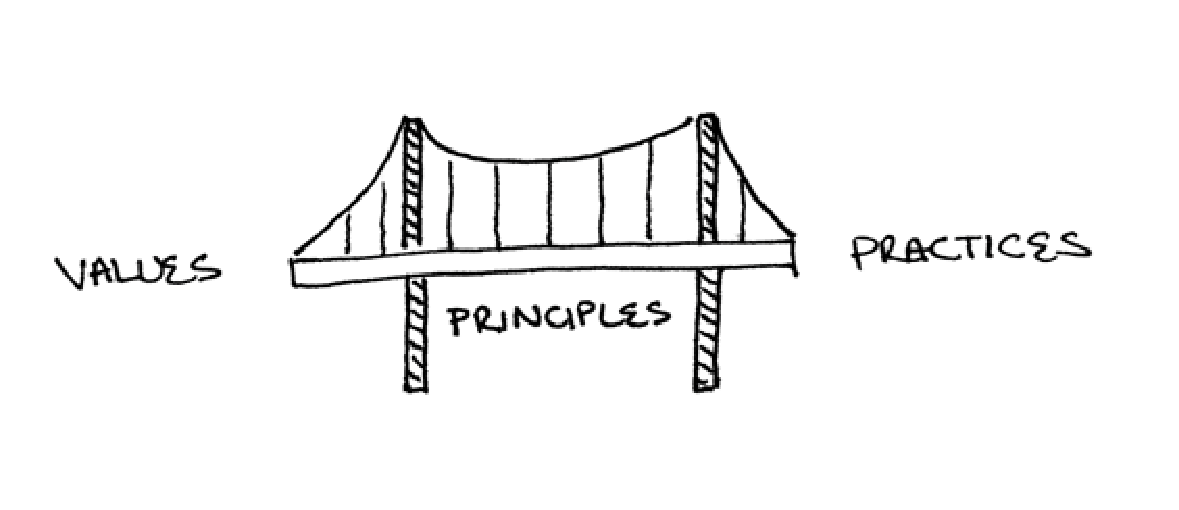
\includegraphics[keepaspectratio=true,scale=0.7]{figuras/fig01.eps}
	\caption{Representação Visual do XP \cite{Beck:2004}}
	\label{fig01}
\end{figure}

A seguir serão descritas características gerais das práticas propostas pela metodologia, fundamentais para o entendimento do ciclo de desenvolvimento do XP.

\section{Práticas}

O conjunto de práticas do XP tem a finalidade de aumentar a produtividade enquanto mantém a qualidade do produto. \cite{Maurer:2002} As práticas são o último elo que compõe a ponte descrita por Kent Beck. A sustentação e travessia da mesma depende de todos os elementos que a compõe. A figura \ref{fig02} mostra um detalhamento das práticas presentes no XP:

\begin{figure}[ht]
	\centering
		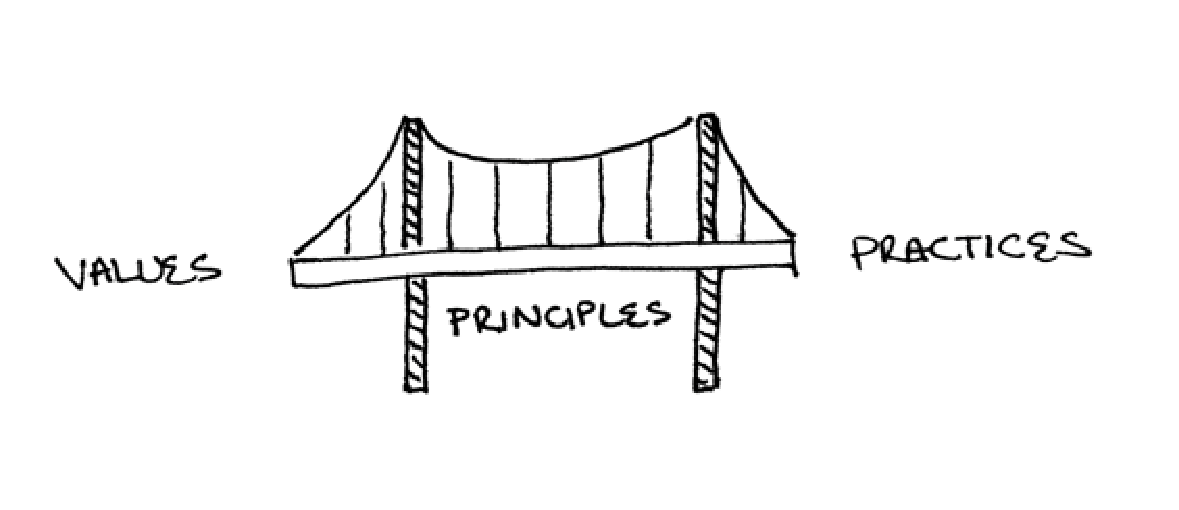
\includegraphics[keepaspectratio=true,scale=0.5]{figuras/fig02.eps}
	\caption{Práticas do XP \cite{Beck:2004}}
	\label{fig02}
\end{figure}

Podemos descrever um número enorme de práticas neste trabalho, entretanto o foco será apenas descrever as práticas mais utilizadas pelo mercado e aquelas que, de alguma forma, agreguem valor à construção de uma metodologia de desenvolvimento baseada no XP.

\cite{Maurer:2002} descreve de forma sucinta as práticas mais utilizadas pelo mercado e mais importantes dentro de um ciclo de desenvolvimento de software:


\begin{itemize}

	\item \textbf{Envolvimento dos \textit{Stakeholders}:} Determinar e priorizar os requisitos é uma prática fundamental para o sucesso de um projeto.  Esta prática envolve agregar valor ao desenvolvimento de software. Conforme as mudanças emergem, os desenvolvedores podem consultar o cliente para entender suas necessidades e prioridades ao invés de especular através de uma documentação robusta o que seria a prioridade.

	\item \textbf{Pequenas Versões:} Devido a mudança constante de requisitos, o XP mantém ciclos com pequenas versões para garantir que cada das mesmas produza um software com valor ao cliente. Ciclos pequenos com lançamento de pequenas versões reduz os riscos e permite a adaptação dos desenvolvedores as mudanças dos requisitos.

	\item \textbf{Metáfora:} Uma metáfora representa uma visão do sistema que pode ser compreendida por ambas as partes, tanto técnica quanto de negócios. Geralmente é uma ideia que representa as funcionalidades básicas do sistema a ser desenvolvido.

	\item \textbf{Testes:} Teste são uma parte fundamental do XP. Sejam testes de aceitação desenvolvidos pelos clientes, ou testes unitários construídos pelos desenvolvedores do software. Todos eles têm a função de prevenir erros e guiar os desenvolvedores  na validação da funcionalidade após o código escrito.

	\item \textbf{Projeto Simples:} O XP não prevê esforço no desenvolvimento de uma solução robusta para um problema. Resolver os problemas de hoje, evitando redundâncias, com o menor número de classes e métodos possíveis é o objetivo do desenvolvedor. Códigos com um design simples facilitam a manutenção sem a necessidade de documentação extensa. Isso evita predições erradas sobre o produto, além do gasto de recursos para refatoração.

	\item \textbf{Refatoração:} A refatoração pode ser considerada como qualquer mudança que melhore a manutenibilidade e o entendimento do código fonte, mas não alterando a funcionalidade do mesmo. \cite{Fowler:1999} A refatoração é um fator importante dentro do projeto devido ao fato da pouca documentação. O código deve ser de simples entendimento e compreensão, assim como a forma mais simples de código para que os testes escritos rodem.

	\item \textbf{Programação em pares:} No XP a produção do código é feita por duas pessoas trabalhando em uma única máquina.  Uma pessoa controla  teclado e mouse, pensando na resolução do problema e se aquela abordagem funcionará para determinada situação. A segunda pessoa pensa de forma mais estratégica, avaliando se a solução aplicada é a melhor possível para desenvolver a funcionalidade proposta. As posições são trocadas constantemente durante o dia.

	\item \textbf{Jogo de Planejamento:} O objetivo desta prática é planejar o escopo do próximo ciclo de desenvolvimento. São avaliadas as prioridades dos desenvolvedores e do negócio. São definidas quais funcionalidades mais importantes, quais podem ser postergadas e quais são essenciais para o desenvolvimento do sistema. Ao final do planejamento são definidas as funcionalidades a serem desenvolvidas, de acordo com a experiência do desenvolvedores e com o espaço de tempo para o próximo ciclo.

	\item \textbf{40 horas por semana:} De acordo com a metodologia, nenhuma pessoa pode trabalhar mais de 40 horas por semana sem que sua produtividade seja afetada. Mesmo que os desenvolvedores sejam pressionados a trabalhar além deste período na semana, o resultado, na maioria das vezes é queda de produtividade e qualidade do produto.

	\item \textbf{Propriedade Coletiva de Código:} Todos podem modificar qualquer parte do código a todo o momento. Não existe propriedade individual de nenhum trecho de código. A propriedade coletiva auxilia na troca de conhecimento entre os membros e evita problemas quando algum desenvolvedor deixa a equipe, já que todos os integrantes tem conhecimento de todas as partes do código.

	\item \textbf{Padrões de Codificação:} Padrões de código são uma obrigação em um projeto onde integrantes modificam constantemente partes do sistema. Padrões facilitam o entendimento e a manutenção além de tornar o código consistente.

	\item \textbf{Integração Contínua:} Desenvolvedores devem integrar o código sempre que possível. Integrando o código uma vez ao dia garante que sempre haverá um novo executável com novas funcionalidades para a validação do cliente.

\end{itemize}

Após uma breve explicação das características da metodologia e um aprofundamento em suas práticas, a próxima seção descreve-rá o ciclo de trabalho proposto pelo Extreme Programming.

\section{Visão de Projeto no XP}

O XP deixa o processo de desenvolvimento tradicional de lado. EM vez de analisar, planejar e desenvolver um design visando um futuro muito distante, o XP explora a redução de custos na mudança do software desenvolvendo um pouco de cada uma dessas atividades durante o ciclo de desenvolvimento de software. \cite{Beck:1999} A figura \ref{fig03} ilustra o ciclo de desenvolvimento de um projeto na visão do XP.

\begin{figure}[h]
	\centering
		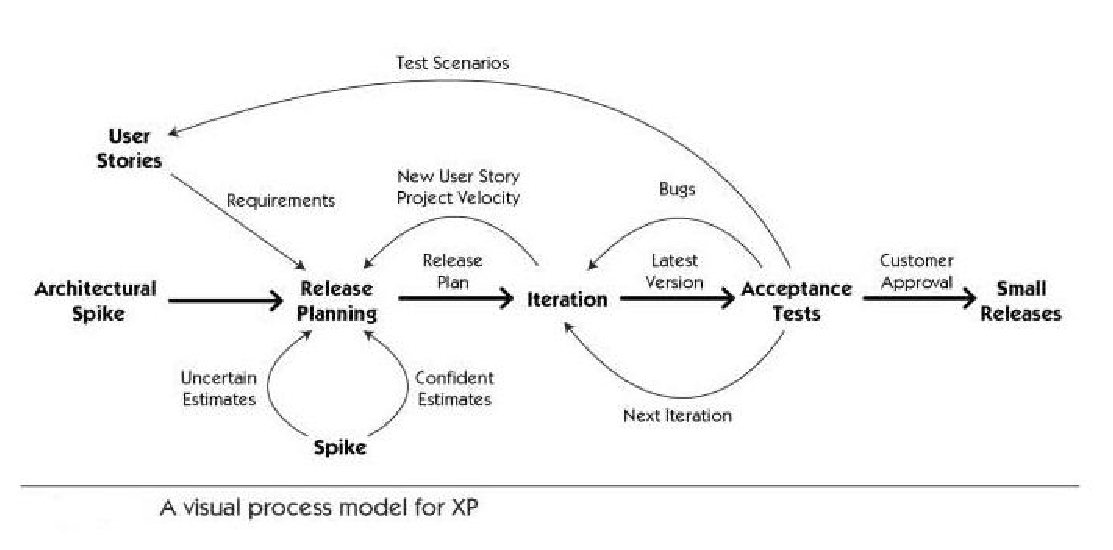
\includegraphics[keepaspectratio=true,scale=0.9]{figuras/fig03.eps}
	\caption{Processo de Desevolvimento XP \cite{Process}}
	\label{fig03}
\end{figure}




\chapter[Tamanho Funcional de Software]{Tamanho Funcional de Software}

Este capítulo descreve o surgimento da contagem de tamanho funcional, a técnica de contagem de pontos de função (IFPUG) pelo manual do CPM.

\section{Tamanho Funcional de Software}

A contagem de tamanho funcional de software surgiu no ano de 1979, com Albrecht. A proposta era estimar o tamanho de um software a partir das funcionalidades entregues ao usuário. Estas primeiras métricas ficaram conhecidas como Function Points(FP)  e  Function Points Analysis (FPA)  e eram uma alternativa para suprir o problema da indústria em estimar prazos e esforço necessário para a o desenvolvimento de software.

Nos anos seguintes surgiram várias propostas de melhoria e variações do modelo apresentado no ano de 1979. No ano de 1986 a International Function Point User Group (IFPUG) foi criada como uma organização sem fins lucrativos. Sua função era, entre algumas outras, a de promover e disseminar o gerenciamento de projetos através do uso de FPA. Em 1996 a International Organization for Standardization (ISO), estabeleceu princípios de comum entendimento e uma interpretação consistente das  definições que permeiam a medição de tamanho funcional. Atualmente a ISO/IEC 20926:2010 regulamenta a análise de pontos de função. Ela define regras e etapas para aplicação da mesma em projetos de desenvolvimento e manutenção de software.

\section{Contagem de Pontos de Função}

O manual de contagem do IFPUG descreve o procedimento de contagem de pontos de função a partir de alguns passos:

\begin{itemize}

\item Definir as fronteiras de medição, o escopo e o propósito da mesma. A fronteira de um software pode ser definida estabelecendo uma fronteira lógica entre o software a ser medido, seus usuários e a interação com outros softwares. Essa fronteira pode ser subjetiva, consequentemente tornando difícil a delimitação do início de um software e do término de outro.

\item Medir as funções de dados. Uma função de dados refere-se aos requisitos na visão do usuário em relação ao armazenamento e a referência de dados da aplicação. Podem ser classificadas em arquivos lógicos interno e externos.

\item Medir as funções de transação. Estas funções são caracterizadas pelo processamento de dados por uma funcionalidade provida ao usuário. Podemos classificá-las em três tipos: saída externa, entrada externa e consulta externa e definir a complexidade de cada uma como baixa, média e alta.

\item Calcular o tamanho funcional. A partir da soma da complexidade das funções da dos e das funções de transação é possível calcular um tamanho total em pontos de função de um software. Vale ressaltar que existem aspectos para ajustar os pontos de função de acordo com a necessidade do projeto.

\item Reportar os resultados. O último passo listado pelo manual corresponde ao relato dos resultados obtidos pela contagem, além de interpretações e possíveis tomadas de decisões a partir dos valores obtidos.

\end{itemize}

A figura a seguir representa os passos descritos anteriormente para a realização do procedimento de contagem de pontos de função:

\begin{figure}[h]
	\centering
	\label{fig04}
		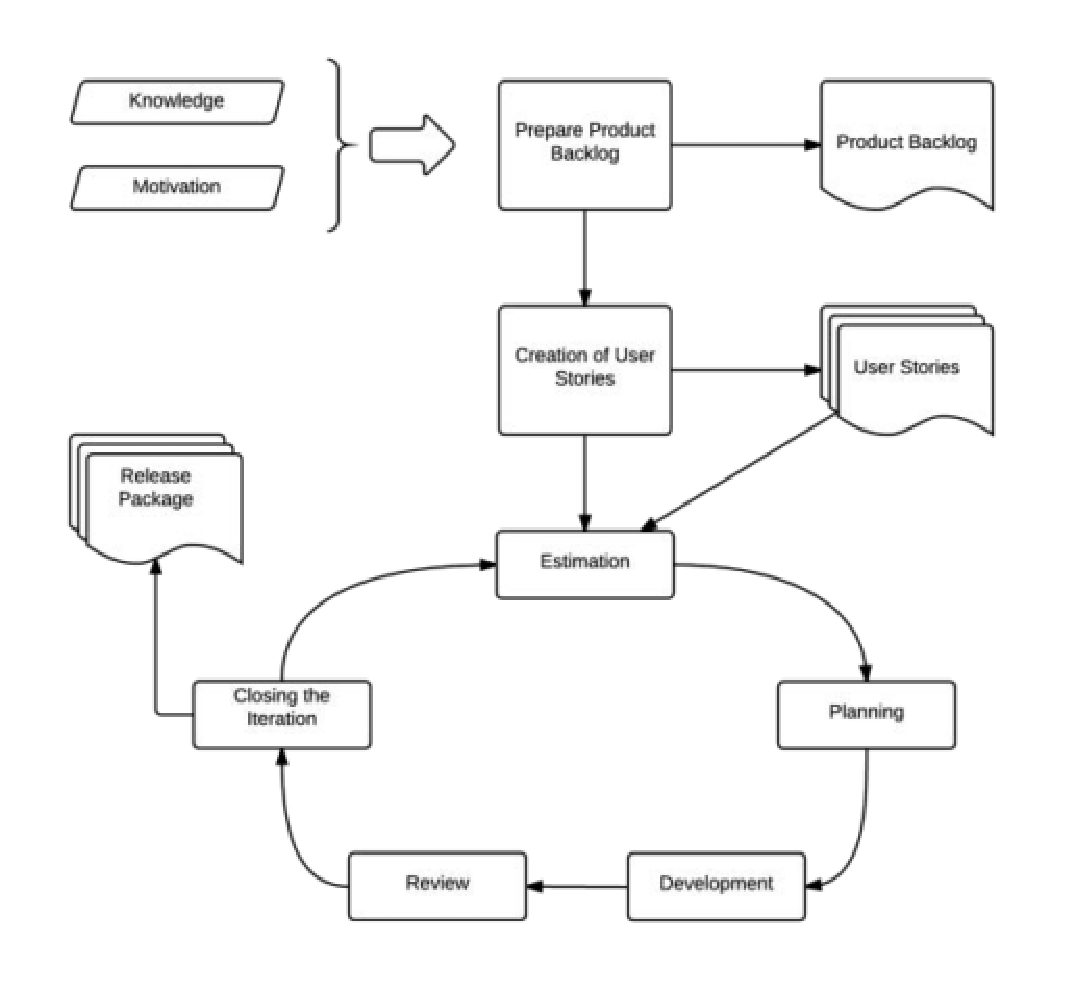
\includegraphics[keepaspectratio=true,scale=0.4]{figuras/fig04.eps}
	\caption{Processo de contagem de pontos de função. Fonte: Roteiro de métricas do SISP}
\end{figure}


As tabelas abaixo descrevem a pontuação de funções de dados e funções de transação de acordo com a complexidades medidas durante a contagem:





Apesar da eficiência da contagem de pontos de função, ao longo dos anos estudos foram feitos a fim de descobrir problemas, lacunas do processo e possíveis melhorias para o mesmo. Buscando saber quais seriam esses problemas e alternativas para solucionar essas lacunas, em 2015 três autores brasileiros realizaram um processo de revisão sistemática na literatura para agrupar as observações feitas por outros autores na área.

Os autores classificaram os problemas encontrados em três tipos: Peso e complexidade, independência de tecnologia e ajuste da pontuação. As principais críticas a parte de peso e complexidade da contagem de pontos de função diz respeito a mesma classificação em complexidade de duas funções de transação ou de dados com diferentes quantidades de campos e referências a arquivos. Outra crítica seria o espaçamento entre as complexidades. Alguns autores acreditam que definir apenas como baixa, média e alta pode ser muito e alto e acabar não detalhando de forma mais aproximada a real complexidade de desenvolvimento de uma funcionalidade.

Problemas relacionados a independência de tecnologia também são citados na revisão sistemática feita pelos autores. O principal questionamento dos pesquisadores é a falta de adaptação do processo de contagem às novas linguagens de programação. A abordagem não reflete o atual desenvolvimento de software, principalmente o advento e crescimento da orientação a objetos. A independência de tecnologias também diz respeito ao hardware, muito diferente hoje do que a existente a 20 anos atrás.

Por fim, o estudo relata problemas como ajuste do ponto de função. Alguns autores afirmam que o ajuste não considera  importantes requisitos não funcionais, dentre eles: usabilidade, manutenibilidade, eficiência, e portabilidade.

Mesmo com os problemas e lacunas descobertos ao longo dos anos, a indústria de desenvolvimento de software continuam usando a contagem de pontos de função para a estimativa de tamanho de software.Na visão de Ebert \cite{Ebert:2014}, as companhias passaram a adotar esse modelo de estimativa com algumas finalidades. A primeira delas seria alocar melhor os recursos a partir de uma primeira estimativa de prazo e esforço necessário para a produção. Outro fator seria a estimativa de esforço quando alguma mudança nos requisitos do projeto ocorresse. Além disso também seria possível medir a produtividade e taxas de entrega de software, possibilitando benchmarks  e análises de pontos de melhoria no processo de desenvolvimento.

A utilização dos pontos de função para estimativas de projeto passou a ser usada também por órgãos de governo e não só por companhias ou fábricas de desenvolvimento de software. O Roteiro de Métricas de Software(2016) do SISP cita essa utilização do processo em órgãos e em empresas privadas, além dos benefícios obtidos por ambos pela utilização dos mesmo:  “Diversas instituições públicas e privadas têm utilizado a métrica Ponto de Função(PF) nas estimativas e dimensionamento de tamanho funcional de projetos de software devido aos diversos benefícios de utilização desta métrica, destacando-se: regras de contagem objetivas, independência da solução tecnológica utilizada e facilidade de estimativa nas fases iniciais do ciclo de vida do software.”
